\section{Broad-to-Narrow Positioning of This Study}
\label{sec:broad_to_narrow_positioning}

The previous section presents the broad taxonomy of blockchain scalability solutions. However, the scope of this report is narrower than the complete scalability landscape. Figure~\ref{fig:broad_to_narrow_zkrollup_positioning} therefore shows the specific broad-to-narrow research path followed in this project. It connects the general blockchain scalability literature to the particular ZK-rollup bottlenecks evaluated by the proposed RollupX benchmarking framework.

\begin{figure}[!htbp]
    \centering
    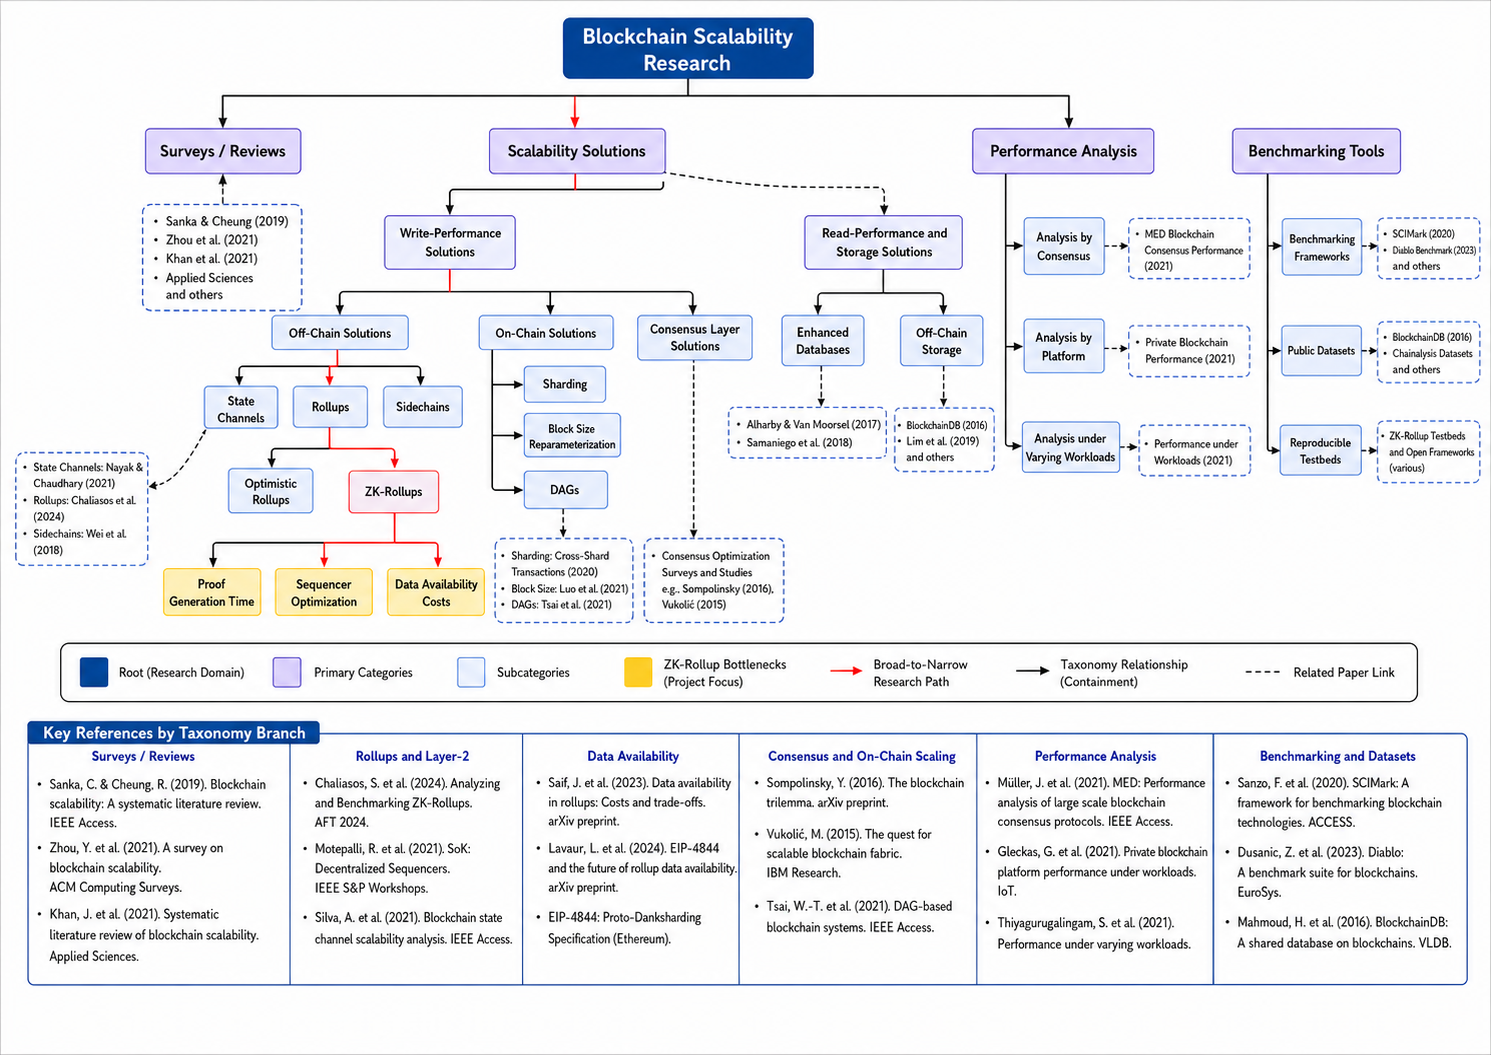
\includegraphics[
        width=0.82\textwidth,
        keepaspectratio
    ]{figures/chapter2/blockchain_scalability_taxonomy.png}
    \caption{Broad taxonomy of blockchain scalability solutions.}
    \label{fig:blockchain_scalability_taxonomy}
\end{figure}

As shown in Figure~\ref{fig:broad_to_narrow_zkrollup_positioning}, blockchain scalability research includes surveys and reviews, scalability solutions, performance analysis, and benchmarking tools. Among these branches, this project is mainly positioned under scalability solutions and performance analysis. The scalability-solution branch explains where rollups fit within the wider design space, while the performance-analysis and benchmarking branches motivate the need for measurable and reproducible evaluation.

The highlighted path in the figure shows how the research scope narrows from blockchain scalability research to scalability solutions, then to write-performance solutions, off-chain solutions, rollups, and finally ZK-rollups. This narrowing is important because the project does not attempt to solve every scalability problem. Instead, it focuses on the part of the scalability problem where transaction execution, batching, proving, data availability, and Layer-1 settlement interact.

Within the rollup branch, the taxonomy separates optimistic rollups from ZK-rollups. This project focuses on ZK-rollups because they use validity proofs to support correctness of off-chain execution. However, ZK-rollup performance depends on several practical system-level factors, not only on the cryptographic proof system. In particular, proof generation time can delay hard finality, sequencer behavior can affect ordering and soft-finality latency, and data availability publication can dominate Layer-1 cost.

Therefore, the final level of the diagram identifies the three bottlenecks studied in this report: proof generation time, sequencer optimization, and data availability cost. These three areas correspond directly to the configurable dimensions of the RollupX prototype. The framework supports controlled experiments over batching and sequencing policies, prover modes, and data availability modes, allowing the project to evaluate their impact on throughput, latency, finalization time, and cost.

This broad-to-narrow positioning also explains the research gap addressed by the project. Existing scalability surveys classify the solution space, and existing production rollup studies provide useful real-world observations. However, production ZK-rollups are difficult to modify, instrument, and evaluate under identical workloads. A modular research-grade prototype is therefore needed to isolate how individual design choices affect ZK-rollup performance in a reproducible setting.
